\documentclass{article}
\usepackage{enumitem}
\usepackage{listings}
\usepackage{amsfonts}
\usepackage{latexsym}
\usepackage{fullpage}
\usepackage{graphicx}
\usepackage{paralist}
\usepackage{tikz-timing}

\lstdefinelanguage{VHDL}{
  morekeywords={
    library,use,all,ENTITY,IS,PORT,IN,OUT,end,architecture,of,
    begin,and, ARCHITECTURE, IF, THEN, SIGNAL,END, PROCESS
  },
  morecomment=[l]--
}

\usepackage{xcolor}
\colorlet{keyword}{blue!100!black!80}
\colorlet{comment}{green!90!black!90}
\lstdefinestyle{vhdl}{
  language     = VHDL,
  basicstyle   = \ttfamily\scriptsize,
  keywordstyle = \color{keyword}\bfseries\ttfamily,
  commentstyle = \color{comment}\ttfamily,	
  tabsize=1
}

\renewcommand{\lstlistingname}{Code}

% Default margins are too wide all the way around. I reset them here
\setlength{\topmargin}{-.5in}
\setlength{\textheight}{9in}
\setlength{\oddsidemargin}{.125in}
\setlength{\textwidth}{6.25in}


%\let\oldenumerate\enumerate
%\renewcommand{\enumerate}{
  %\oldenumerate
  %\setlength{\itemsep}{1pt}
  %\setlength{\parskip}{0pt}
  %\setlength{\parsep}{0pt}
%}


\begin{document}
\title{Organization of Digital Computer Lab \\ EECS112L/CSE 132L}
\author{\textbf{Assignment 4 }\\ \textbf{Multi-Cycle Processor} \\ \\
prepared by: Team Stressed \\ Student name: \\ Mansi Tyagi \\ Student ID: \\23334840\\ \\ Student name: \\ Erik Henriquez\\ Student ID: \\57374677\\ \\ Student name: \\ Kevin Chau \\ Student ID: \\76934313\\ \\ Student name: \\ Steven Chow\\Student ID: \\70916812\\ \\ Student name: \\ Paul Dao \\Student ID: \\30658761\\ \\
EECS Department\\ Henry Samueli School of Engineering \\ University of California, Irvine \\ \\
{February 22, 2016}} 


\date{}
\maketitle


\section{Summary of Processor Design}
\subsection{What We Learned}
A multicycle processor is able to use shorter clock cycles, since it doesn't need to accomodate load word, the slowest instruction. The multicycle processor splits the datapath so that instructions can be read or written into and the ALU can be accessed at each step.

\subsection{Description}
To change from a single-cycle processor to a multicycle processor we needed to eliminate two adders, expand the controller port list, and combine the instruction and data memories. Removing the excess adders reduced the number of costly components the datapath was using. Instead, because of the new datapath, the ALU, which includes an adder, is accessible at every step. The combined memories mimics reality, in which computers have a large memory, rather than two separate memories. This reduces the length of the datapath, increasing the frequency and decreasing the number of cycles. It also ensured that the memory, either instruction or data, could be accessed from any step. The controller signals have been adjusted to accomodate the combined Instruction and Data Memory to include a IorD signal, which indicates which memory values need to be stored or accessed from.

\subsection{Testbench Architecture}
For the most part, our testbench is maintaining the same cycles as it did for the single-cycle processor, simply because we didn't have time to change it. However, since we are now implementing a multicycle processor, different instructions will require different amounts of time to complete. Jump and branch instructions are the fastest instructions, requiring 3 cycles, while load word is the slowest at 5 cycles.


\section{Sample Program}
	
\subsection{Simulation Waveform}
\bfseries{After designing and testing our Processor, we generated the following waveforms:} \\ \\
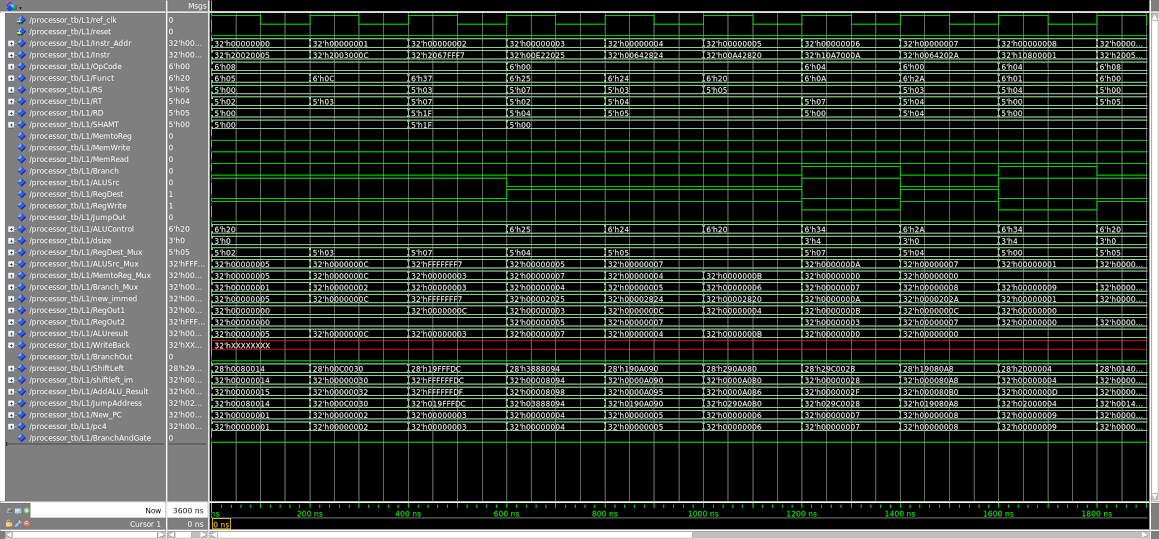
\includegraphics[width=0.8\textwidth]{waveform_part1.png} \\ \\
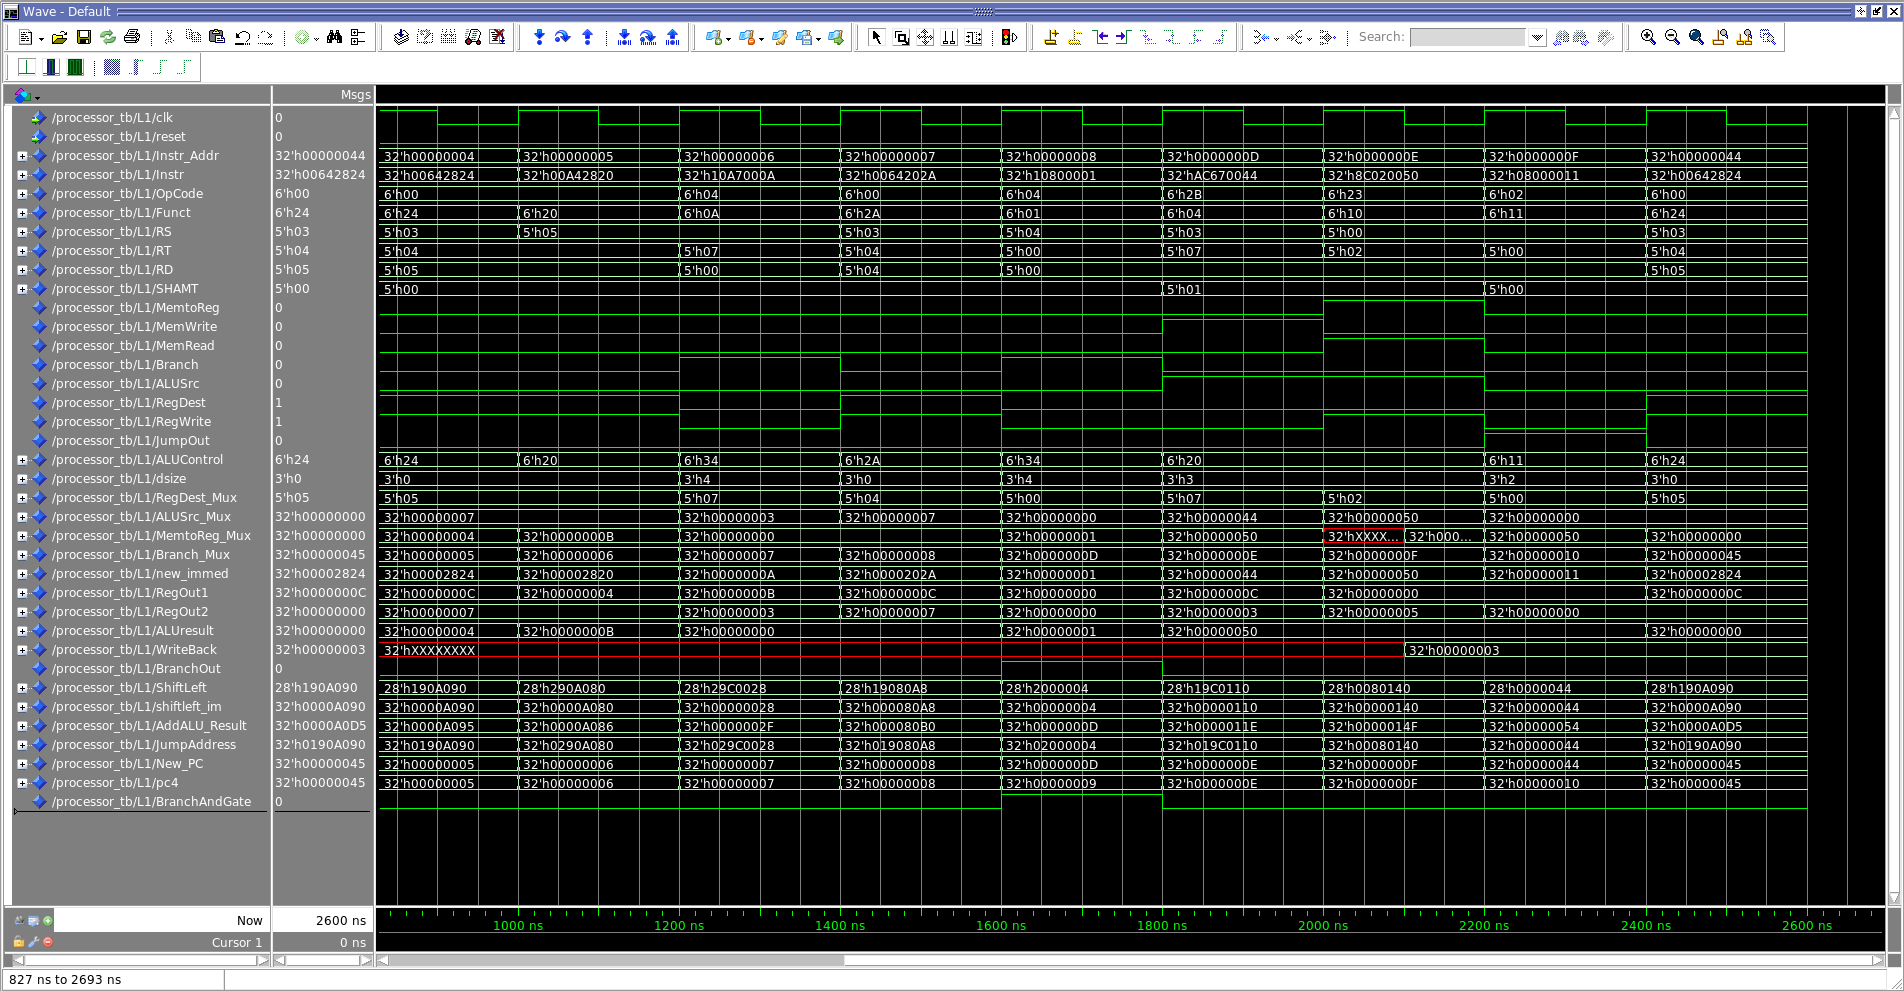
\includegraphics[width=0.8\textwidth]{waveform_part2.png} \\

As you can see, our branch and jump instructions worked as expected. Of the 18 instruction in the example program, only 12 were actually executed. We included a 13th cycle in our waveform to display the "garbage" instruction after our jump instruction.


\section{Synthesis}
We were unable to finish synthesizing the multicycle processor we created.


\section{Known Issues} 
Due to our unfamiliarity with SystemVerilog, we chose not to use the testbench to preload instruction memory. For the Questasim simulation, we read the example program instructions from a file.  For synthesis, we created a second version of instruction memory that has instructions preloaded into memory in order to synthesize the Processor properly.
\\


\section{Conclusion}
As a multicycle processor, our project supports the full MIPS instruction set and allows faster instructions to use shorter clock cycles.


\end{document}
